\section{Lupus disease prediction}

This experiment involves real data gathered by "Lupus Clinic", Reumatologia, Università Sapienza, Roma. The data consists in 413 patients. For each patients are available the records of the visits such patience has done in time. For an in-depth description of the data we refer the reader to the work of Francesco Morelli, from which we start our analysis. In his thesis, "Tecniche di apprendimento automatico per la classificazione di pazienti affetti da Lupus" he performed a statical analysis of the data: only the first visit of each patience is considered with the aim to classify a patience as affected or unaffected by the disease at the time of the visit. This analysis led also to the identification of a subset\footnote{Hashimoto, APS , npsle, arterialthrombosis, MyasteniaGravis, FM, age} of features which appear to be the most relevant for the prediction. Our goal is slight different: we aim to predict whether a patience will develop the lupus disease before it is evident from organic damage, i.e. the SDI (systemic damage index) is zero). This is done considering not only the first visits of a patience but his complete history.

For the purpose of this thesis, the important things to underline are that essentially two. The first one is that,  although each visits is described with a fixed number real and binary features, the number of visits  is not the same for each patience. This make RNNs one of few model suitable for this task. The other important thing to notice is that the visits are not equally spaced in time, they can be distanced by a month as by a few years. This is an important difference with all of the tasks we considered until now. Think for example of the polyphonic music prediction where each of the songs is split in equally spaced time beats.

\paragraph{Experiment setup}
We used as \textbf{positive} examples all the patients which are negative at the first visit but results positive in later visits (i.e. we exclude completely all the patients which are positive from the first visit). We use as training sequences only the visits in which the patients has zero SDI .
For the \textbf{negative} examples we choose only the patients which satisfy some temporal constraints. The first requirement is for the recorded history of a patience to be long enough to be able to leave out the last part of it from the training sequence. This ensures that we train the model to give a prediction valid, at least, for such given span of years. We measure this time (in years) with the parameter \texttt{upper span age}.  We than require the remaining part of the visits (which are the only ones used in the training sequence) to cover a sufficiently long period of time with the parameter (in years) \texttt{lower span age} and to be composed by at least \texttt{min visits} number of visits.

\tikzstyle{rnn_style}=[shorten >=1pt,auto,node distance=0.5cm,
thick,
sdi/.style={rectangle,fill=white!50,node distance=0.7cm, draw=none,minimum size=0.5cm,font=\sffamily\normalsize},
missing/.style={circle,fill=white!50,draw,minimum size=0.7cm,font=\sffamily\Huge\bfseries},
label/.style={node distance=0.9cm and 4cm,rectangle,fill=white!50,draw=none,minimum size=0.7cm,font=\sffamily\normalsize},
thick_edge/.style={line width=1.2pt},
thin_edge/.style={line width=0.5pt}
]
\begin{figure}[h]
	\centering
	\begin{tikzpicture}[rnn_style]
	
	%SDI column
	
	\node[sdi]    (x1)[]   {$0$};
	\node[sdi]    (x2)[above of=x1]   {$0$};
	\node[sdi]    (x3)[above of=x2]   {$0$};
	\node[sdi]    (x4)[above of=x3]   {$0$};
	\node[sdi]    (x5)[above of=x4]   {$0$};
	\node[sdi]    (x6)[above of=x5]   {$0$};
	\node[sdi]    (x7)[above of=x6]   {$0$};
	\node[sdi]    (x8)[above of=x7]   {$0$};
	\node[label]  (sdiLabel)[above of = x8] {SDI};
	
	%AGE column
	
	\node[sdi]    (y1)[right =0.5cm of x1]   {$20$};
	\node[sdi]    (y2)[above of=y1]   {$21$};
	\node[sdi]    (y3)[above of=y2]   {$22$};
	\node[sdi]    (y4)[above of=y3]   {$25$};
	\node[sdi]    (y5)[above of=y4]   {$30$};
	\node[sdi]    (y6)[above of=y5]   {$35$};
	\node[sdi]    (y7)[above of=y6]   {$40$};
	\node[sdi]    (y8)[above of=y7]   {$45$};
	\node[label]  (sdiLabel)[above of = y8] {AGE};
	
	\node[label] (arr) [left = 0.7cm of x5] {last training visit};
	
	\draw[decorate,decoration={brace,raise=8pt,amplitude=6pt}, thick]
	(x1.center)--(x5.center) node [black,midway,xshift=-0.7cm, align=center, text width = 3cm] {
		training visits (at least \texttt{min visits})};
	
	\draw[decorate,decoration={brace,raise=8pt,amplitude=6pt, mirror}, thick]
	(y5.center)--(y8.center) node [black,midway,xshift=3.5cm] {
		\texttt{upper span age}};
	
	\draw[decorate,decoration={brace,raise=8pt,amplitude=6pt, mirror}, thick]
	(y1.center)--(y5.center) node [black,midway,xshift=3.5cm] {
		\texttt{lower span age}};
	
	\path[->]
	(arr) edge []  node[]{} (x5);
	
	
	\end{tikzpicture}
	\caption{Example of a negative training sequence.}
	\label{fig:lupus_neg_example}
\end{figure}

We normalized all the data to be in range (0,1).
We explored all the combination for \texttt{upper span age} in [1, 2], \texttt{lower span age} in [1, 2], \texttt{min visits} in [2, 3, 4, 5]. Since the number of available patients is not big enough to allow a split in train and test set, we repeated the training procedure eight times with different splits of train e test then we put together the predictions on the eight test sets.  The results are shown in Table \ref{table:exp_res}. We repeated the experiment twice: on time with all the features and next with the subset of selected features.

\begin{table}[!h]
	\centering
	\begin{tabular}{c  c  c | m{2cm}  m{2cm} |  c  c}
		upper span age & lower span age & min visits & auc roc score all feats & auc roc score subset feats& pos & neg\\
		\hline
		1 & 1 & 2  & x & 0.62 & 43 & 127\\
		1 & 1 & 3  & x & 0.71 & 43 & 118\\
		1 & 1 & 4  & x & 0.74 & 43 & 107\\
		1 & 1 & 5  & x & \textbf{0.77} & 43 & 87\\
		2 & 1 & 2  & x & 0.65 & 43 & 87\\
		2 & 1 & 3  & x & 0.70 & 43 & 83\\
		2 & 1 & 4  & x & 0.75 & 43 & 67\\
		2 & 1 & 5  & x & 0.75 & 43 & 48\\
		1 & 2 & 2  & x & 0.71 & 43 & 86\\
		1 & 2 & 3  & x & 0.69 & 43 & 85\\
		1 & 2 & 4  & x & 0.73 & 43 & 84\\
		1 & 2 & 5  & x & 0.76 & 43 & 74\\
		2 & 2 & 2  & x & 0.67 & 43 & 44\\
		2 & 2 & 3  & x & 0.71 & 43 & 43\\
		2 & 2 & 4  & x & 0.74 & 43 & 41\\
		2 & 2 & 5  & x & 0.75 & 43 & 35\\
		
	\end{tabular}
	\caption{AUC ROC score for different training sets. Best score in bold.}
	\label{table:exp_res}
\end{table}


\begin{figure}[h]
	\centering
	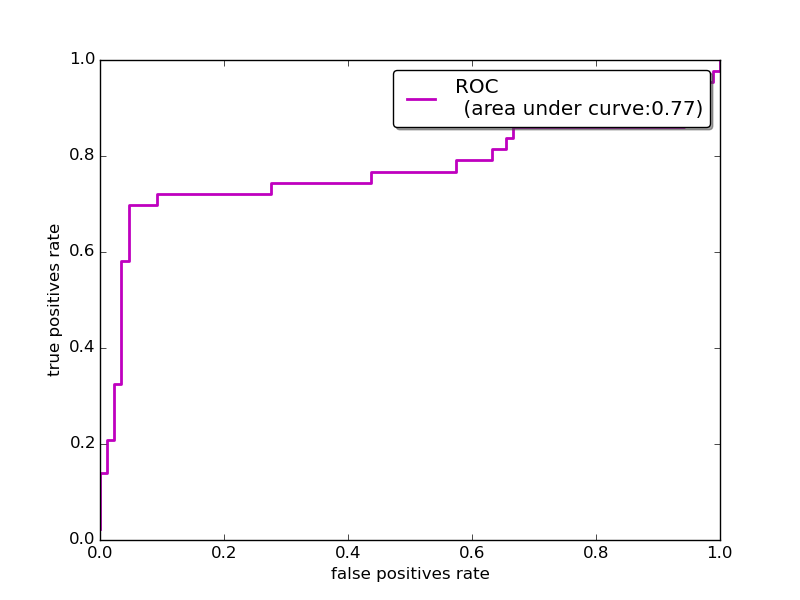
\includegraphics[width= 0.8\textwidth]{chapter4/roc.png}
	\caption{roc curve for the best model}
	\label{fig:roc_best}
\end{figure}

\begin{figure}[h]
	\centering
	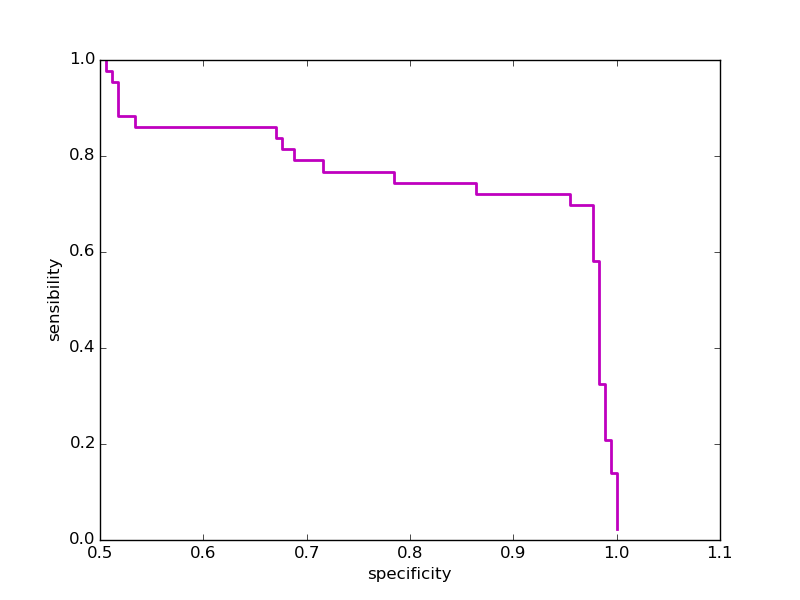
\includegraphics[width= 0.8\textwidth]{chapter4/sensibility_specificity.png}
	\caption{sensibility-specificity curve for the best model}
	\label{fig:sensibility_specificity_best}
\end{figure}

\begin{figure}[h]
	\centering
	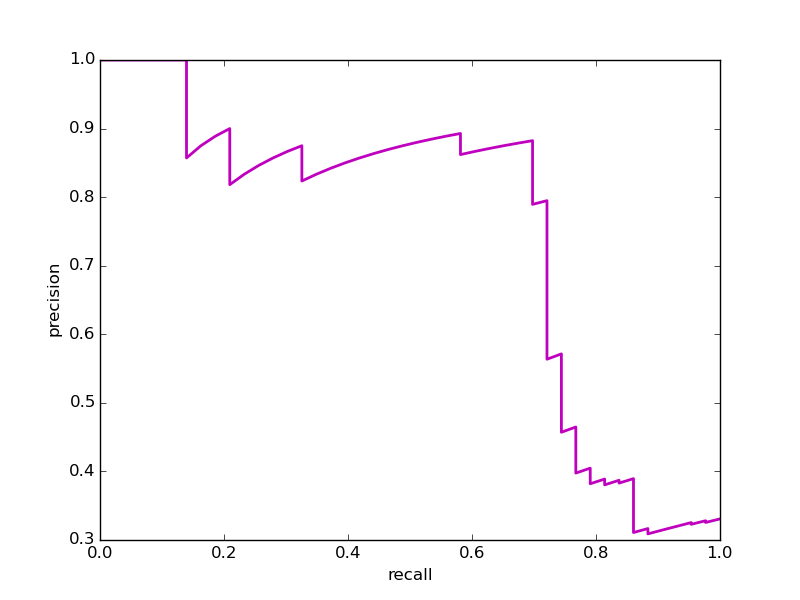
\includegraphics[width= 0.8\textwidth]{chapter4/precision_recall.png}
	\caption{precision-recall curve for the best model}
	\label{fig:precision_recall_best}
\end{figure}

\paragraph{Analysis}
From the results seems clear that using the selected features...
